\documentclass[10pt,a4paper]{article}
\usepackage[a4paper, left=3cm, right=3cm, top=3cm, bottom=3cm, headsep=10mm, footskip=12mm]{geometry}
\usepackage[T1]{fontenc}
\usepackage[ngerman, english]{babel}    % mehrsprachiger Textsatz
% babel: letzte Sprache in Optionen zeigt die Sprache des Dokumentes
% und kann durch den Befehl \selectlanguage{} geaendert werden
% Passen Sie die Optionen des babel-Paketes nach Bedarf an!
\usepackage{float}
\usepackage{graphicx}
\usepackage{pdflscape}
\usepackage{mathtools}
\usepackage{amssymb, amsmath, amstext}
\usepackage{amsthm}
\usepackage{xcolor}
\usepackage{nameref}
\usepackage{siunitx}
\usepackage{makecell}
\usepackage{hyperref}
\usepackage{enumitem}
\usepackage[superscript,biblabel]{cite}
\usepackage{caption}
\usepackage{subcaption}
\usepackage{tabularx} 			% Tabellen erzeugen
\usepackage{multirow}			 % Zeilen in Tabellenbearbeitung
\usepackage{multicol} 			% Spalten in Tabellenbearbeitung 
\usepackage{lmodern}                        % Ersatz fuer Computer Modern-Schriften 
\usepackage{amsmath}                                           % zum besseren Aussehen am Bildschirm
\usepackage{booktabs} % für schönere Tabellen
\usepackage{sidecap}
\usepackage{rotating} % für die Landscape-Umgebung
\usepackage{afterpage}
\definecolor{Bluetitle}{HTML}{1F3864}
\definecolor{Greyish}{HTML}{5A5A5A}
\renewcommand{\refname}{Reference}
\usepackage{array,multirow}
\newcommand{\specialcell}[2][c]{%
	\begin{tabular}[#1]{@{}c@{}}#2\end{tabular}}




\begin{document}
	
	\begin{titlepage}
		\begin{center}
			\begin{figure}[h!tbp]
				
\includegraphics[width=\linewidth]{HUlogo.PNG}
			\end{figure}
			\vspace*{0.5cm}
			
			\textcolor{Bluetitle}{\textbf{\huge Qualitative und quantitative Charakterisierung
					der Photosynthesepigmente}}\par
			
			\vspace*{1.4cm}
			
			\textcolor{Greyish}{\textbf{Versuchsdurchführende}}\par
			\textcolor{Greyish}{Oscar Moore (634083)}\par
			\textcolor{Greyish}{Frido (....)}\par
			\textcolor{Greyish}{Philipp.. (...)}\par
			\textcolor{Greyish}{Daniel... (...)}\par
			\textcolor{Greyish}{Huyen Anh Nguyen (572309)}\par
			\vspace*{0.5cm}
			\textcolor{Greyish}{\textbf{Versuchsort}}\par
			\textcolor{Greyish}{Campus Nord, Haus 9}\par
			\textcolor{Greyish}{R2002}\par
			\vspace*{0.5cm}
			\textcolor{Greyish}{\textbf{Versuchsbetreuer}}\par
			\textcolor{Greyish}{Prof. Dr. rer. nat. Bernhard Grimm}\par
			
			\vspace*{1.0 cm}
			
			\textcolor{Greyish}{11. Juni 2024}\par
			
			\vspace*{1.0 cm}
			
			
		\end{center}
		
		\tableofcontents
		
	\end{titlepage}
	
	
	\section{Einführung}
	

	
	\section{Material und Methode}
	Für diesen Versuch wurde die Tabakpflanze Nicotiana tabacum als Wildtyp und die antisense FC1 mutierte Variante verwendet.
		\subsection{Herstellung des Pigmentextraktes}
		\subsection{Photometrische Bestimmung Chlorophylle a und b}
		\subsection{DC-Trennung Chlorophylle und Carotinoide}
		Das Pigmentextrakt im basischen Aceton wurde jeweils vom Wildtyp-Extract und Mutanten-Extract 5 mL entnomen und mit 1 mL Petrolether versetzt und 3 mal vorsichtig invertiert.
		Die Proben wurden für 10 Minuten im Eis inkubiert und die obere dunkelgrüne Phase für die weiteren Versuchen entnommen.\\
		\\
		50 Mikroliter von den beiden Proben wurden auf einer Dünnschichtchromatographi-Platte (agekürzt: DC-Platte) als breite Bande aufgetragen.
		In einem mit Laufmittel (Petrolether/Aceton/Isopropanol/Wasser, 400:80:48:1)-abgesättigte DC-Kammer wird die DC-Platte inkubiert und der Lauf wurde gestoppt, als diese 5 mm Abstand zur DC-Plattenkante erreicht hatte.
		\subsection{Fluoreszenz des Chlorophyllextractes}
		\subsection{Phäophytinbildung}
	
	\section{Ergebnis}
		\subsection{Quantitative Bestimmung der Pigmente}
			
			\begin{figure}[H]
				\centering
				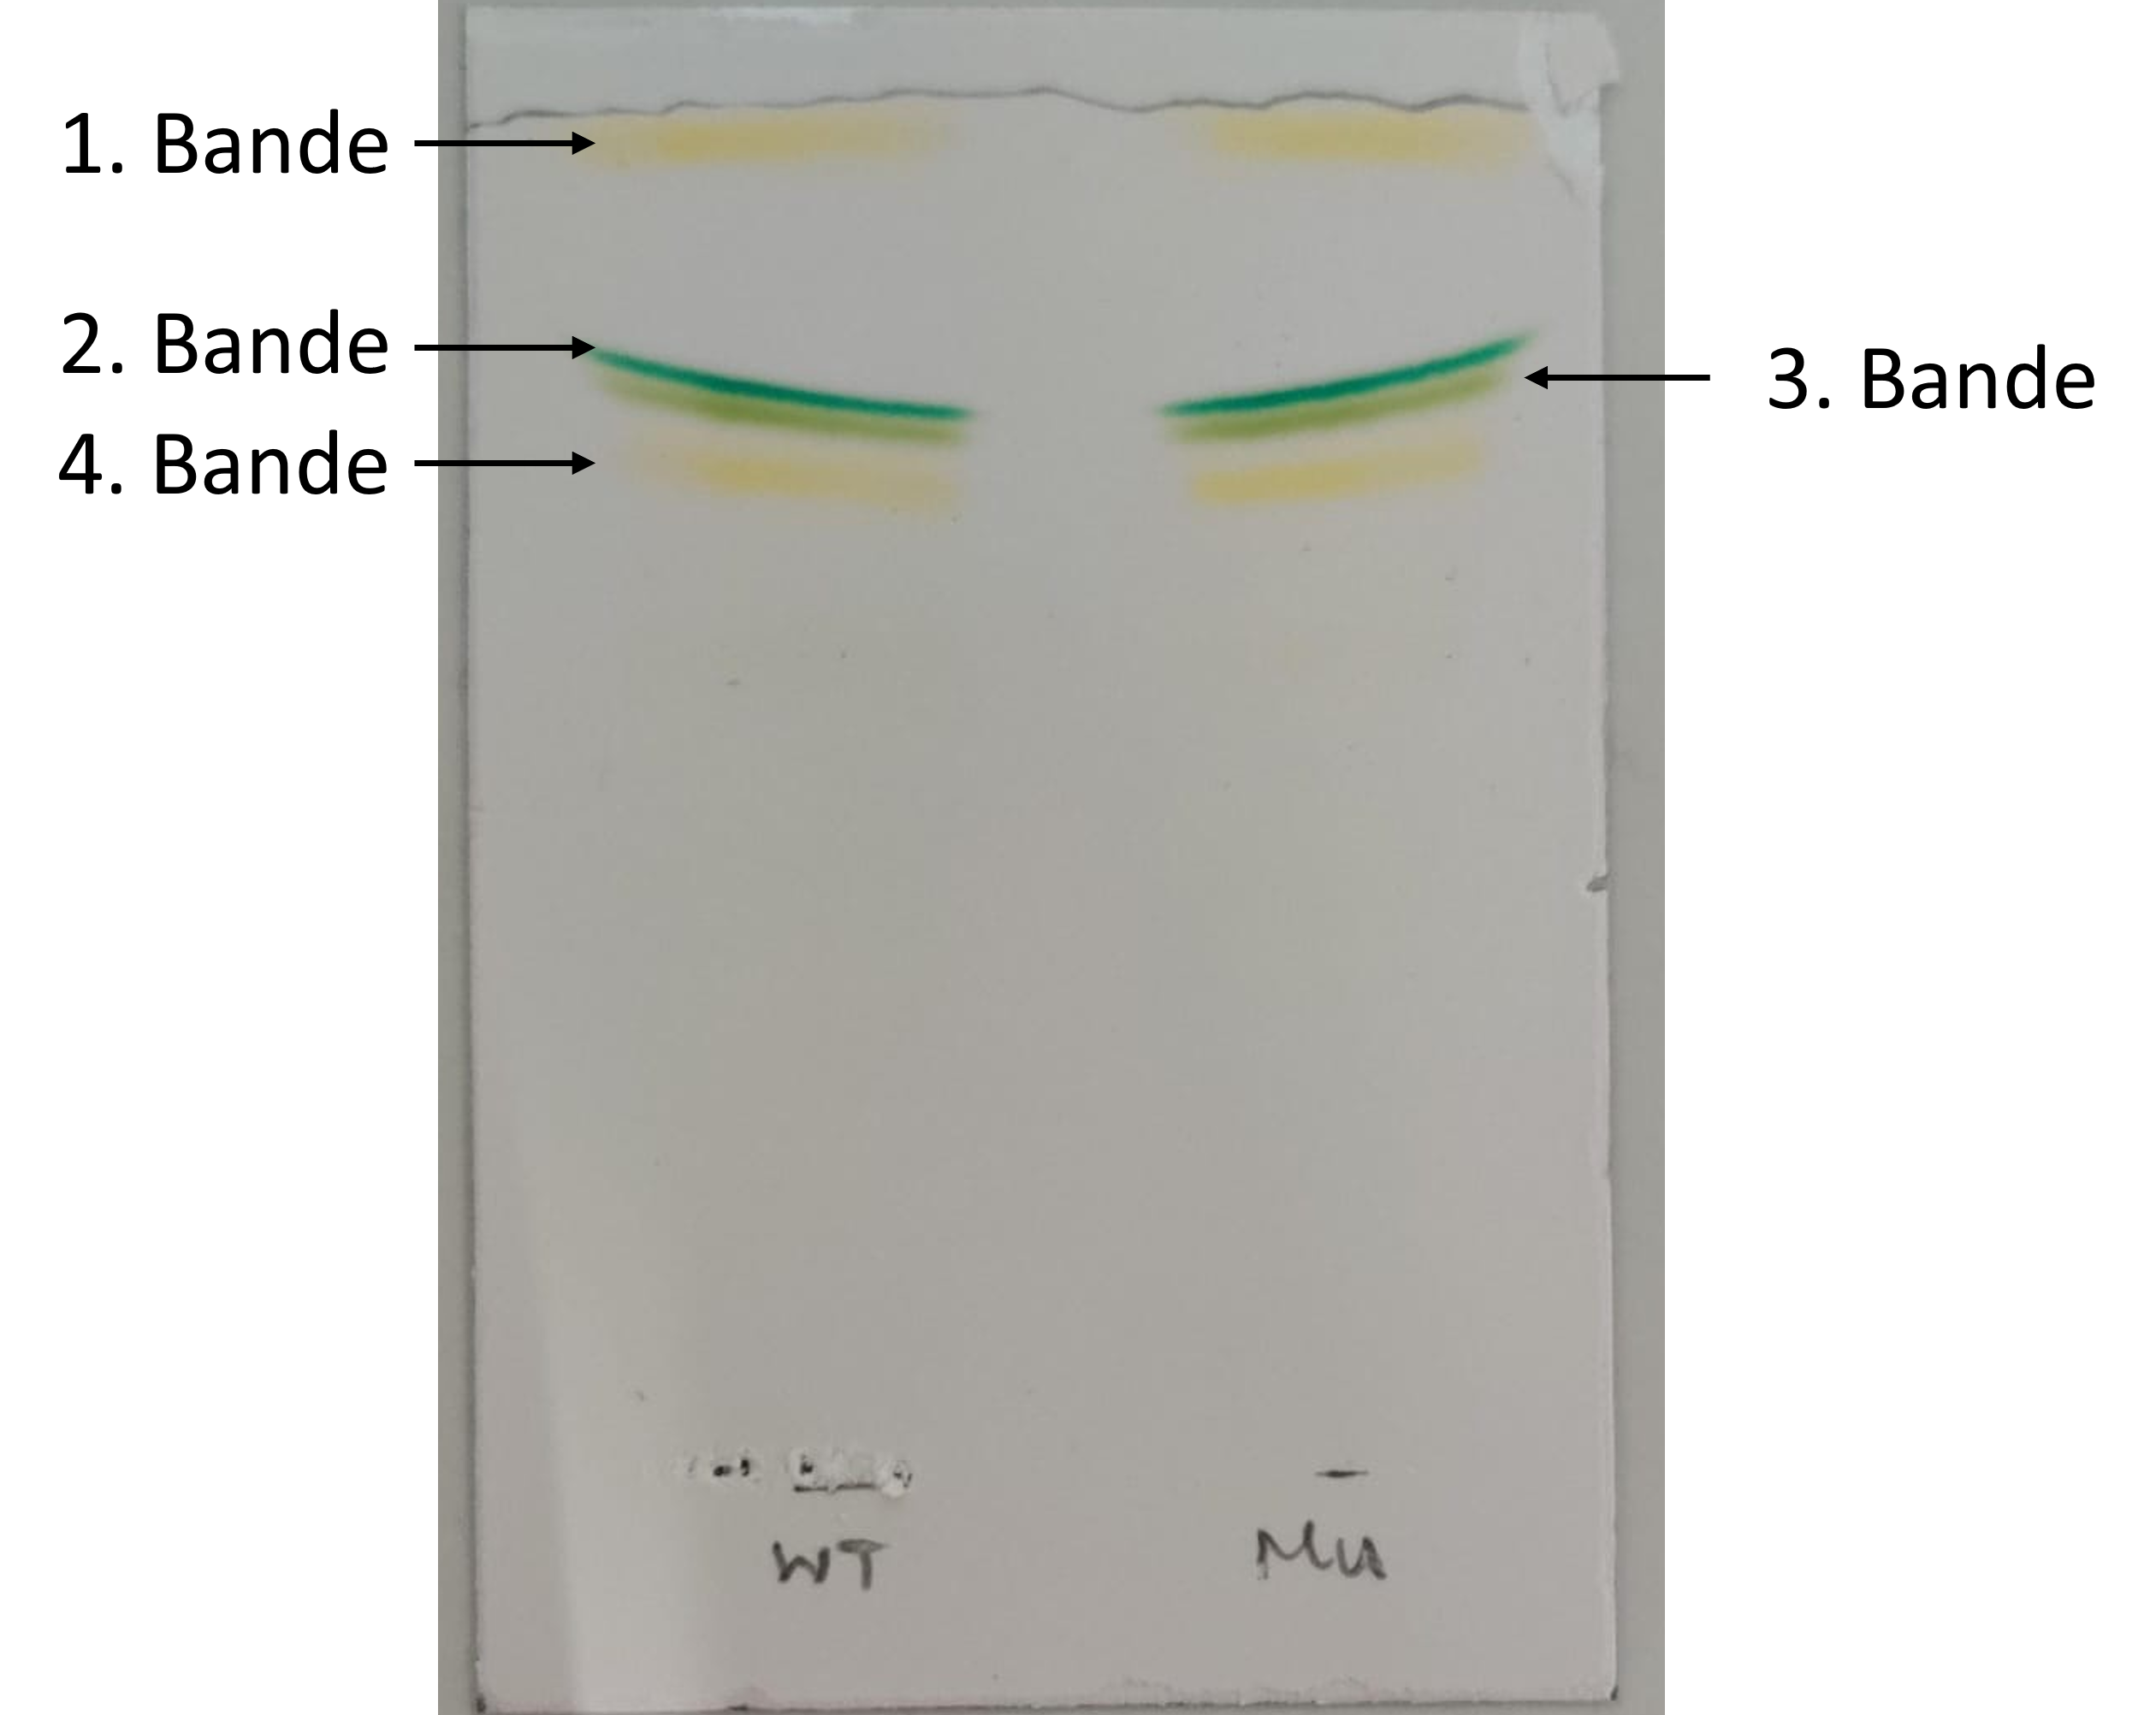
\includegraphics[scale=0.65]{DC-Plate_with_label.png}
				\caption{Probenauftrennung mittels Dünnschicht Chromatographie-Platte von der Spezies Nicotina tabacum (Wildtyp und FC1 - Mutant). Pigment wurden in Petrolether überführt und auf die Platte aufgetragen.}
				\label{fig:DC_Platte}
			\end{figure}
	
			\begin{figure}[H]
				\centering
				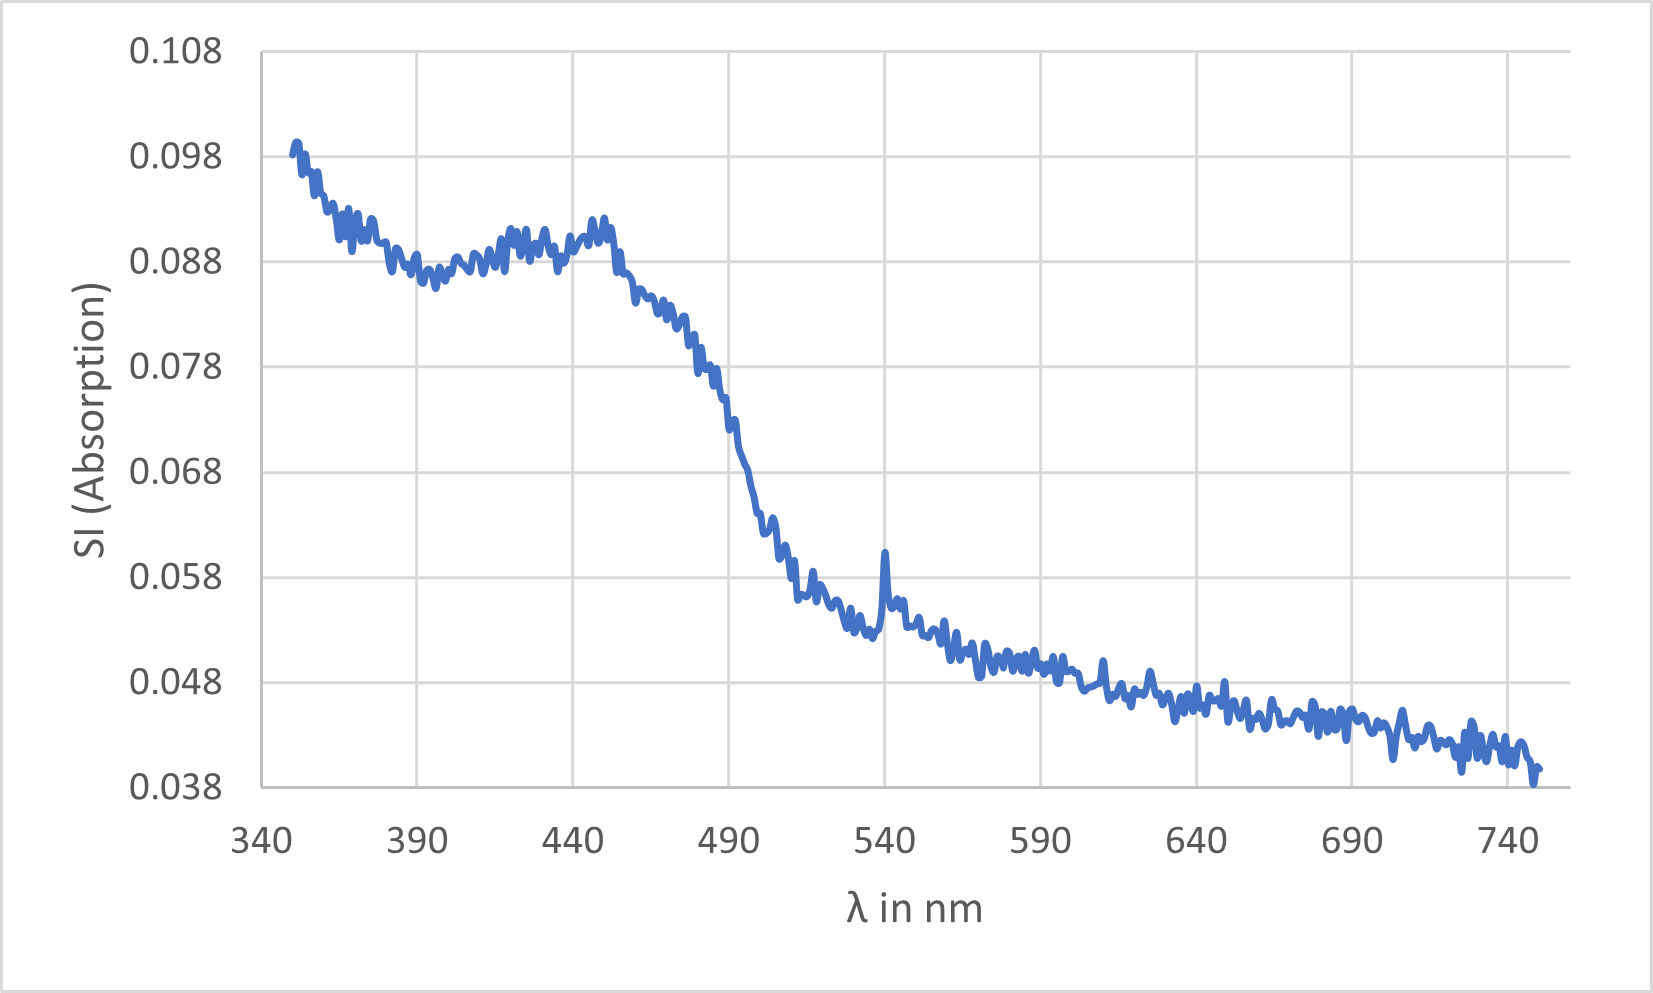
\includegraphics[scale=1]{firstband_axischange.png}
				\caption{}
				\label{fig:erste Bande}
			\end{figure}
			
			\begin{figure}[H]
				\centering
				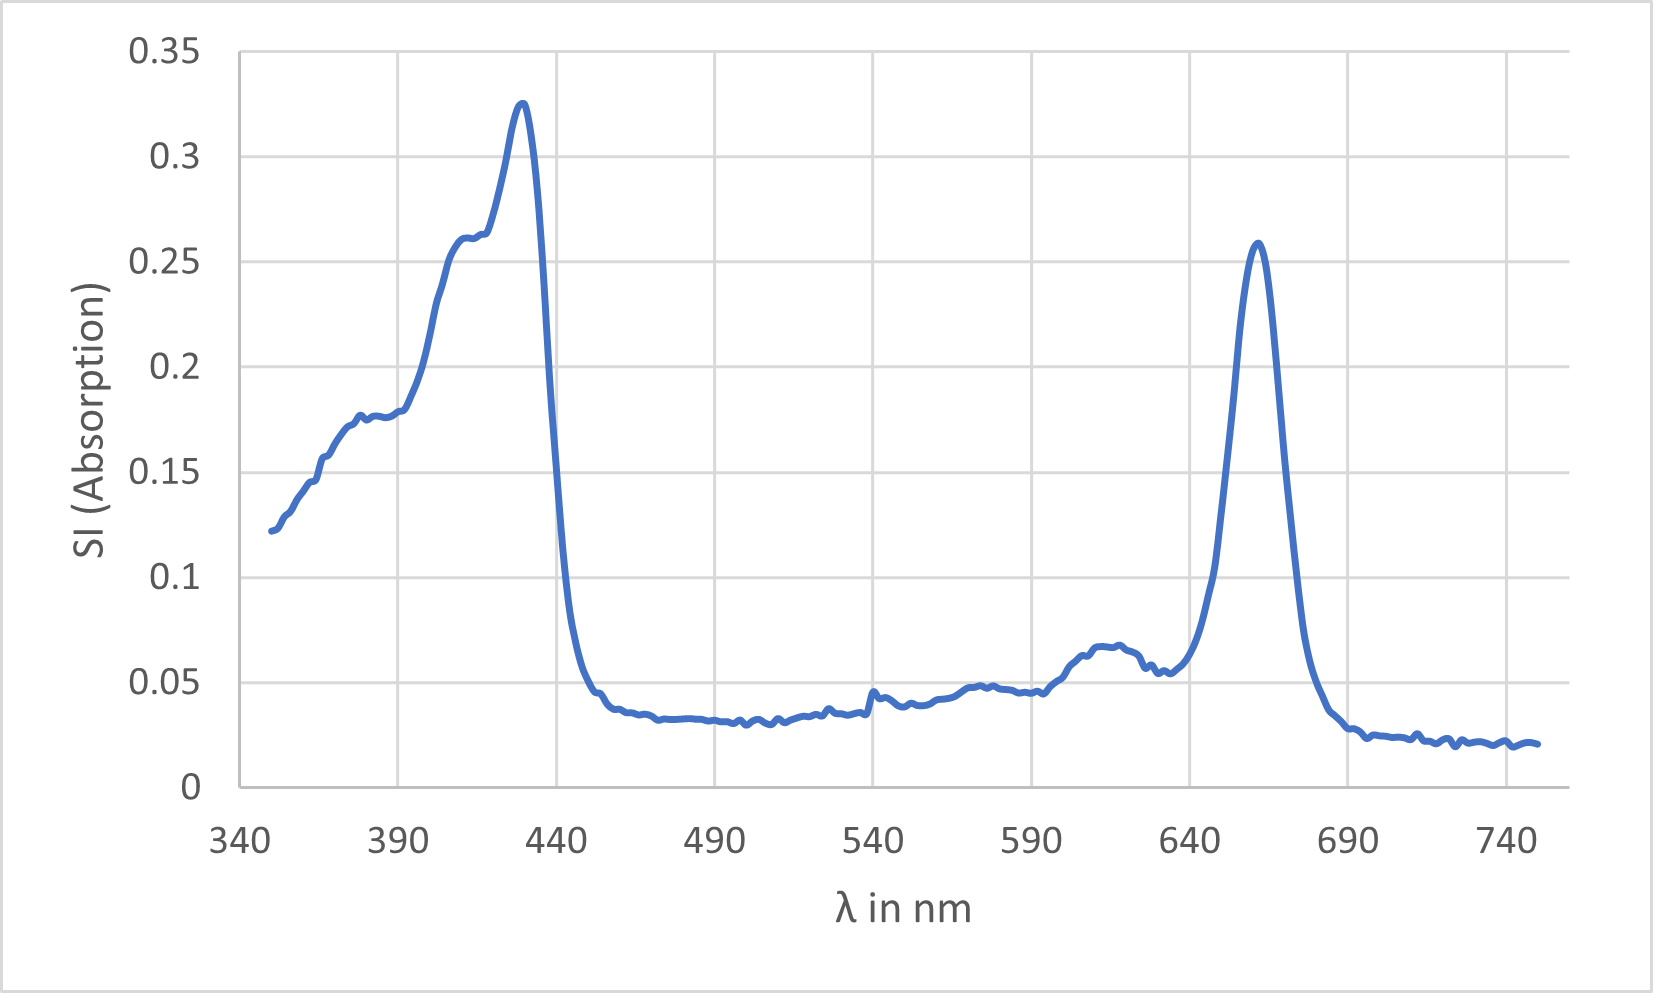
\includegraphics[scale=1]{secondband.png}
				\caption{}
				\label{fig:zweite Bande}
			\end{figure}
			
			\begin{figure}[H]
				\centering
				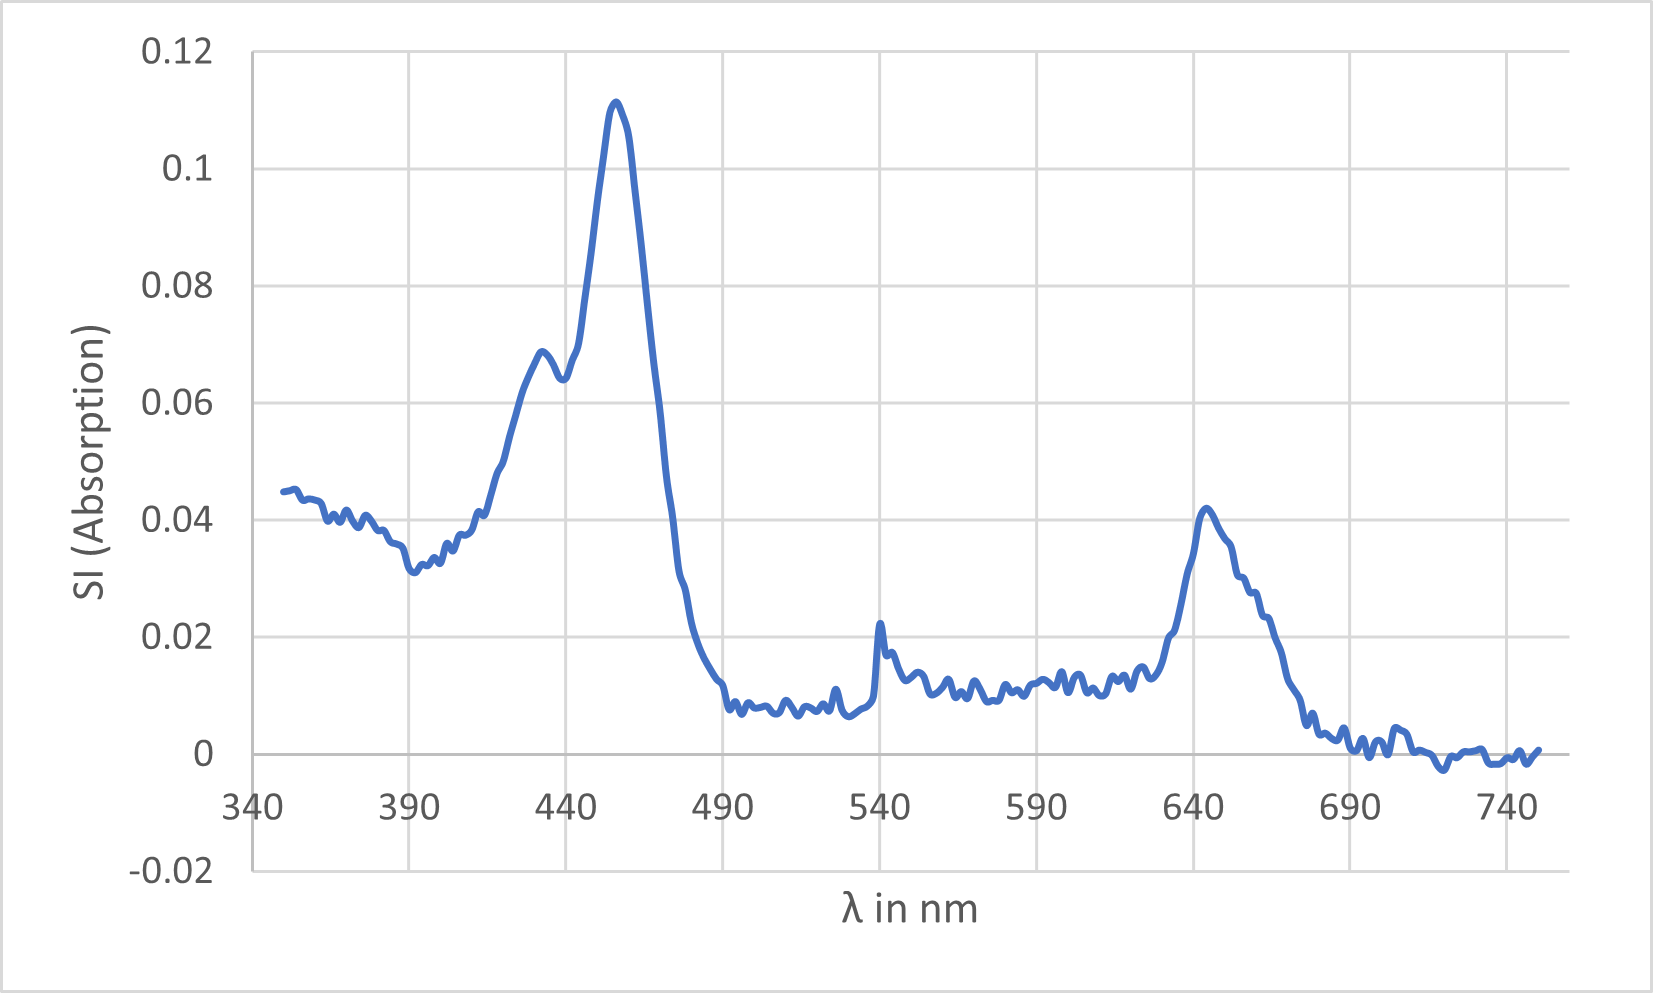
\includegraphics[scale=1]{thirdband.png}
				\caption{}
				\label{fig:dritte Bande}
			\end{figure}
			
			\begin{figure}[H]
				\centering
				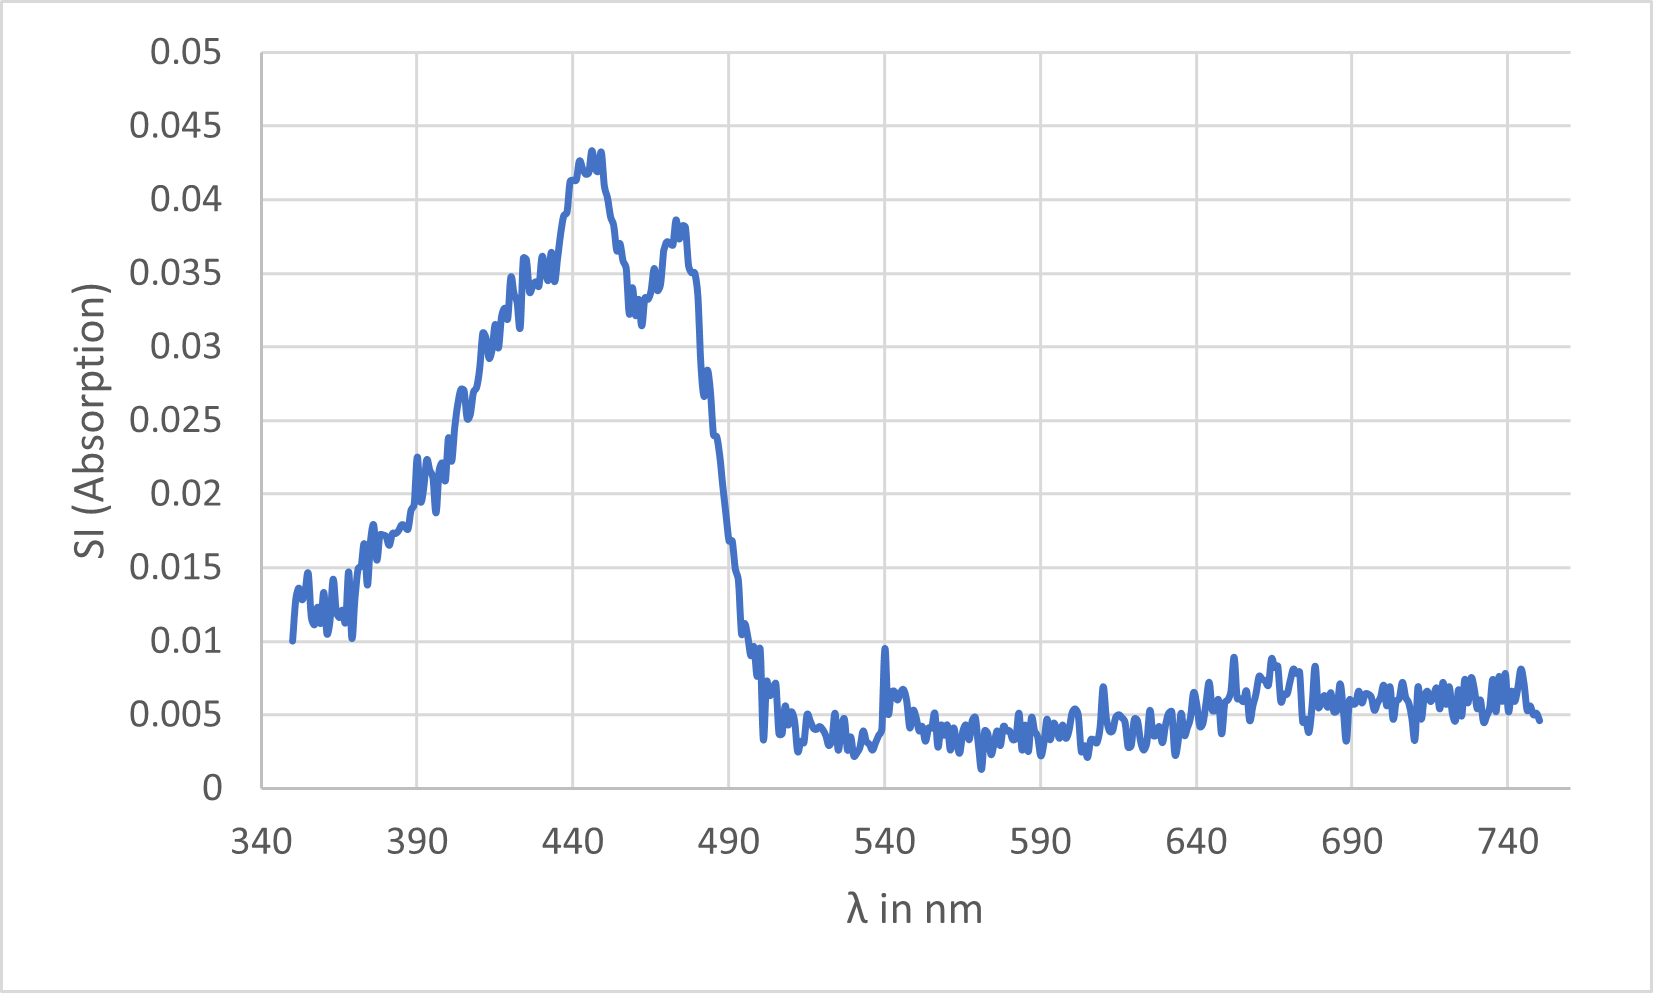
\includegraphics[scale=1]{fourthband.png}
				\caption{}
				\label{fig:vierte Bande}
			\end{figure}
			
			\begin{figure}[H]
				\centering
				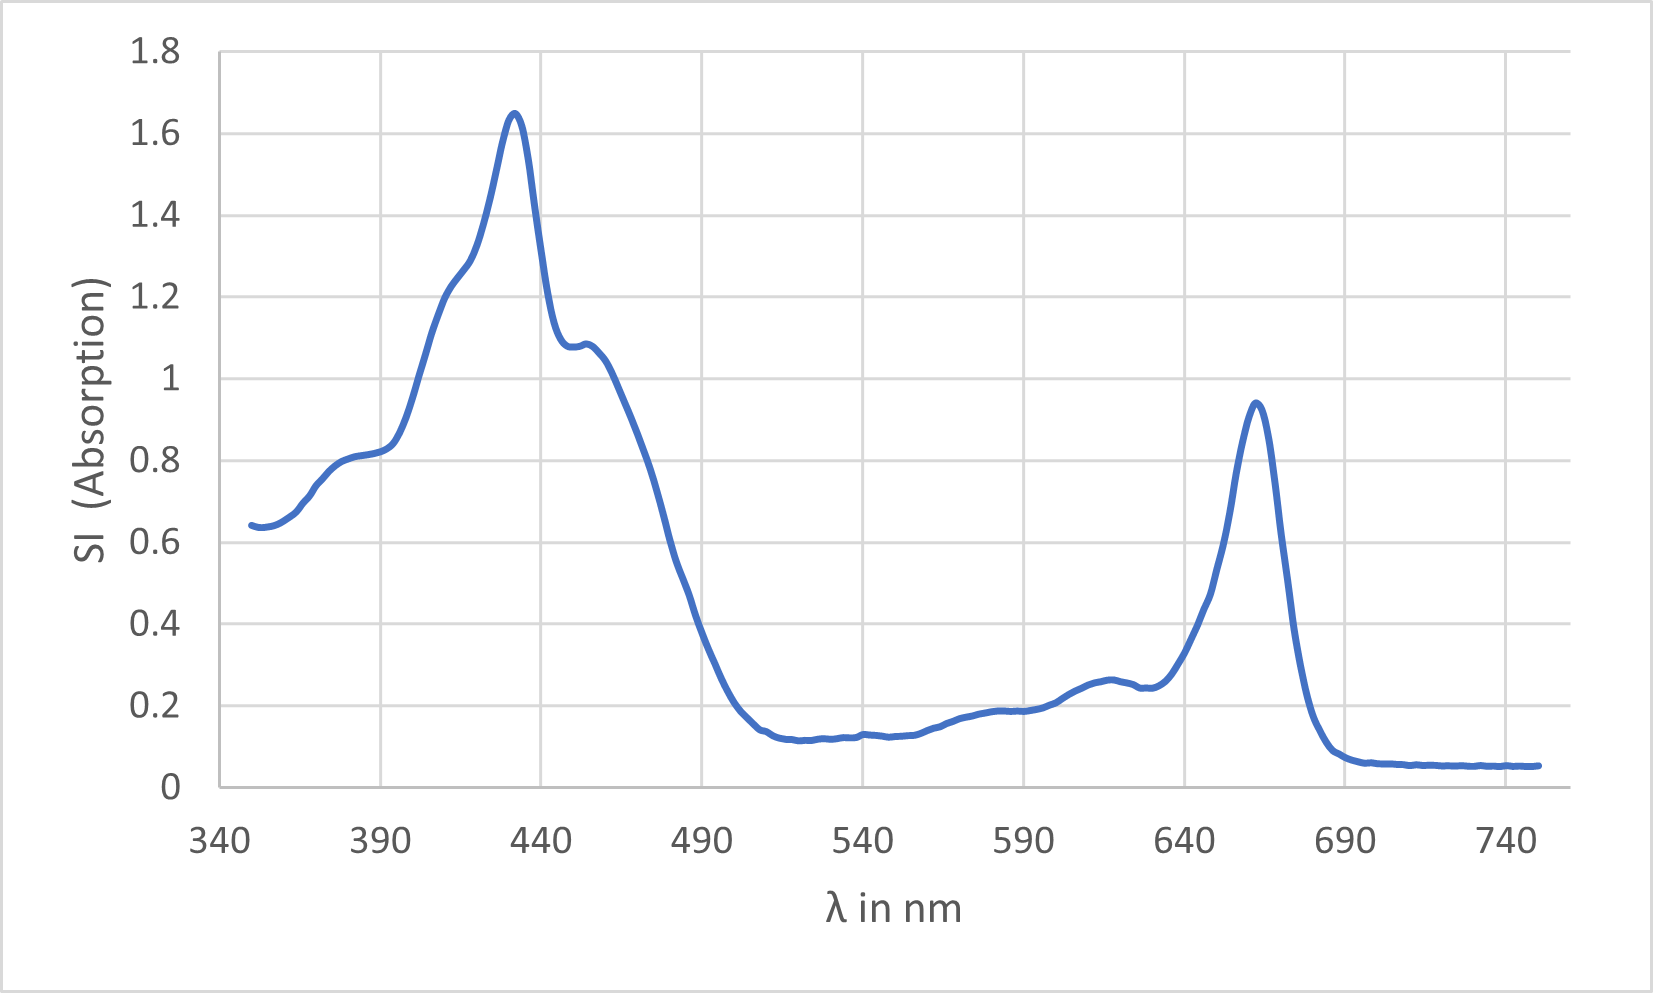
\includegraphics[scale=1]{fifthband.png}
				\caption{}
				\label{fig:fünfte Bande}
			\end{figure}
			
			\begin{figure}[H]
				\centering
				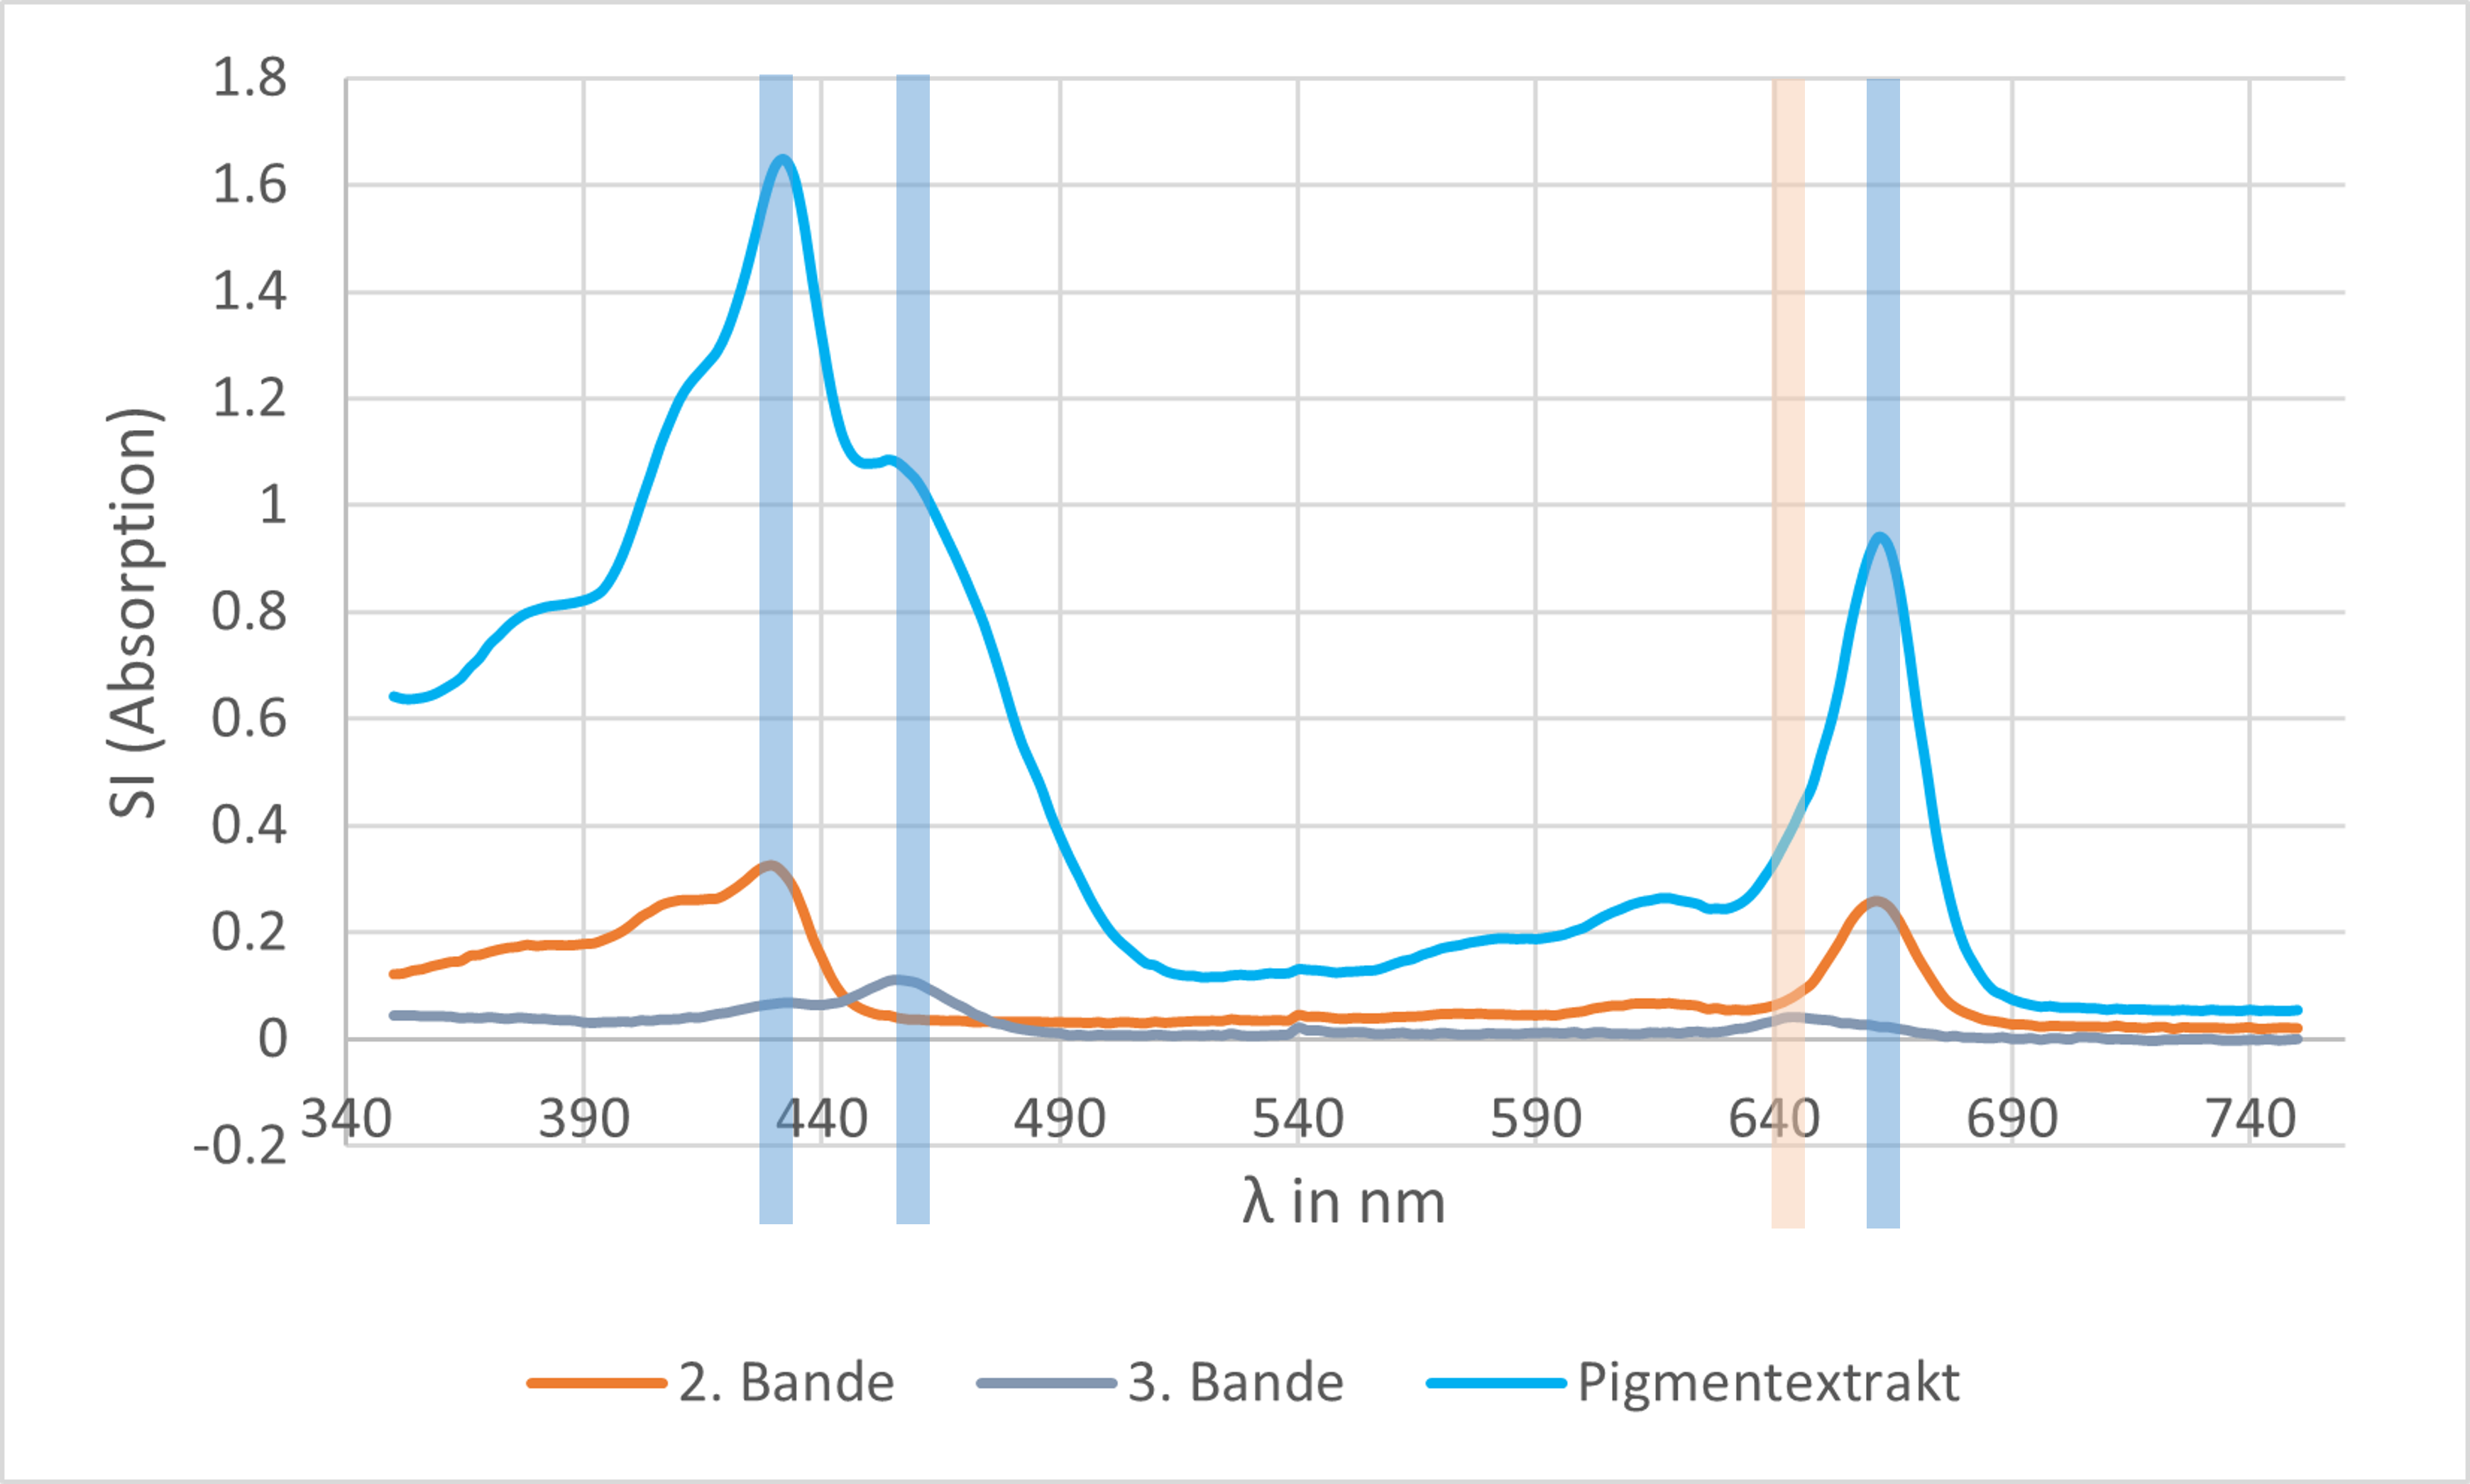
\includegraphics[scale=0.5]{combinedwithcommonpeaks_Pigmentextrakt.png}
				\caption{}
				\label{fig:kombinierteabsorptionsspektrum}
			\end{figure}
			
			
				
	\section{Diskussion}
	
	
	
	
	
	\section{Anhang}
		\subsection{Rohdaten}
			\subsubsection{Einwaage der Proben}
				\begin{table}[H]
					\centering
					\caption{Masse der Blätter und das Volumen des in basischen Aceton extrahierten Pigmenten vom Nicotiana tobacum des Wildtyps und FC1-Antisense Mutant}
					\label{tab:Probemassen und Volumen}
					\begin{tabular}{ccc}
						\toprule
						&Wildtyp& Mutant\\
						\midrule
						m(Frischgewicht) in g & 0.9965 & 0.9960\\
						V(Rohextrakt) in mL & 11.5 & 8\\
						\bottomrule
					\end{tabular}
				\end{table}
				
			\subsubsection{Extinktion des Rohextraktes}
				\begin{table}[H]
					\centering
					\caption{Die Extinktion des Rohextraktes vom Wildtyp und Mutant in basischen Aceton wurde bei $\lambda$ = 470, 646, 663, 720 nm gemessen. Als Blank wurde die Extraktionslösung (100$\%$ Aceton und 20 mM NH$_4$OH) verwendet.
					Die Proben wurden jeweils 1:5 mit der Extraktionslösung verdünnt.}
					\label{tab:Rohdaten Extinktion Rohextraktes}
					\begin{tabular}{ccccc}
						\toprule
						$\lambda$ in nm &470& 646 & 663 & 720\\
						\midrule
						Wildtyp &0.424 & 0.178 & 0.463 & 0.012\\
						Mutant & 0.423 & 0.188 & 0.493 & 0.014 \\
						\bottomrule
					\end{tabular}
				\end{table}
			
			\subsubsection{Substanzstrecke auf der DC-Platte}
				\begin{table}[H]
					\centering
					\caption{Substanzstrecke der 4 Banden aus Figure \ref{fig:DC_Platte} für den Wildtyp (WT) und der FC1-Mutante (MU). Die Laufmittelfront-Distanz beträgt 6.2 cm}
					\label{tab:Distance_Rf_Werte_Banden_Rohwerte}
					\begin{tabular}{cc}
						\toprule
						Substanzstrecke Wildtyp in cm& Substanzstrecke Mutant in cm\\
						\midrule
						6 & 6\\
						4.9 & 4.9\\
						4.5 & 4.5\\
						3.8 & 3.8\\
						\bottomrule
					\end{tabular}
				\end{table}


	\bibliographystyle{unsrt}
	\bibliography{Literatur}
	\newpage
	
\end{document}